\documentclass[10pt,a4paper]{article}
\usepackage[margin=2.2cm]{geometry}
\usepackage{amsmath,amssymb,graphicx,booktabs,caption,float,xcolor,enumitem}
\usepackage[colorlinks=true,linkcolor=blue!50!black,urlcolor=blue!50!black]{hyperref}
\captionsetup{font=small,labelfont=bf}
\setlist{itemsep=1pt,topsep=3pt}
\graphicspath{{figures/}}
\newtheorem{result}{Result}

\title{\textbf{Proofs, co-retention and finite sizes}\\[2pt]
\textbf{in the fact-flow model}}
\author{Claude (theory work, \nolinkurl{analysis/theory_claude/phenomenological_fact_flow/})}
\date{28 October 2026}

\begin{document}
\maketitle

\begin{abstract}
\noindent
This report continues the fact-flow model of 27 October (\nolinkurl{2026-10-27_fact_flow_model}) and answers two
questions: can proofs explain why the symmetric setups reverse at shorter memory than the no-proof setups, and what are
the model's effective finite sizes?

\emph{Proofs.} Replacing the independence approximation by the exact chance of holding all facts of a proof together
raises proof holding a great deal: up to 26 times for 6-fact proofs. The model's proof shares then come close to the
simulator's, but the crossover still does not move. The simulator shows why: there, too, almost nobody holds a complete
proof near the crossover (1--3\% of agents). Completed proofs cannot be what moves the symmetric crossover. The model
points to a different candidate, how strongly the agents' own evidence argues against the wrong answer, to be tested
next.

\emph{Finite sizes.} At short memory, only about 3 of the swarm's 15--18 starting facts survive in an episode, each in
7--9 board copies. The model assumes all 16 circulate, in 2--4 copies. The relevant finite size is therefore the
\emph{number of surviving distinct facts}, an emergent, memory-dependent quantity, not the swarm's 24 agents or its 18
starting facts as such.
\end{abstract}

\section{Proofs with co-retention}
\paragraph{The change.} On 27 October, the chance that an agent holds a complete proof of the correct answer was
approximated by $z=1-(1-m_A^{\ell})^P$. Here $m_A$ is the chance of holding one agent fact, $\ell$ the number of facts in
a proof and $P$ the number of alternative proofs. The proof sizes are taken from the worlds: $(\ell,P)=(6,12)$ in
task003 and $(3,2)$ in Object Placements. The approximation $m_A^\ell$ treats the facts of a proof as held independently.
But one read can bring several of them at once, so they are held together more often.

We replace $m_A^\ell$ by the exact chance $h_\ell$ of holding all $\ell$ facts. The facts are treated as interchangeable,
each with board share $p=b_A/F_A$. Let $h_k$ be the chance of holding $k$ given facts of the proof ($h_0=1$). Then
\begin{equation}
\dot h_k=-k\gamma\,h_k+\sum_{j=1}^{k}\binom kj\,p_k(j)\,\big(h_{k-j}-h_k\big),\qquad
p_k(j)=\sum_{i=0}^{j}(-1)^i\binom ji\big(1-(k-j+i)\,p\big)^{q},\label{eq:h}
\end{equation}
where $p_k(j)$ is the chance that one read of $q$ posts brings exactly a given $j$ of the $k$ facts. In words:
\begin{itemize}
\item the $k$-set is lost when any of its facts is forgotten, at rate $k\gamma$;
\item it is completed when a read brings all the missing ones.
\end{itemize}
This is the ChatGPT agent's recurrence for a fixed board, specialised to equal copies and applied on the model's
changing board. For $k=1$ it reduces exactly to the model's memory equation (a check that passes). The proof variable
becomes $z=1-(1-h_\ell)^P$.

\paragraph{Results} (expectations logged before the run):
\begin{itemize}
\item \textbf{Co-retention raises proof holding: met.} $h_\ell/m_A^\ell$ is 26 for 6-fact proofs and 2.7 for 3-fact
  proofs at $\rho=0.25$, and 6.2 and 1.7 at $\rho=0.5$. The 3-fact values are close to those the ChatGPT agent measured
  in the simulator (1.8--2.6).
\item \textbf{The crossover moves to shorter memory with proofs: not met.} It stays at $\rho=0.25$--$0.3$
  (Fig.~\ref{fig:proofs}a).
\end{itemize}

\begin{figure}[h]
\centering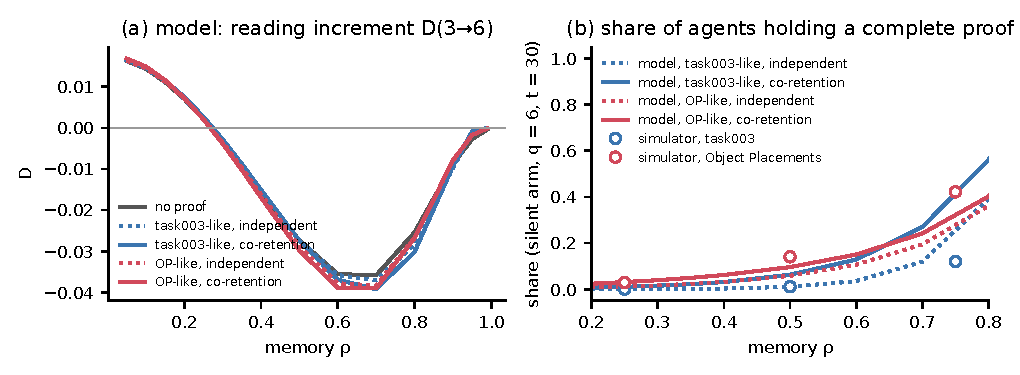
\includegraphics[width=\linewidth]{fig1_proofs.pdf}
\caption{\textbf{Proofs in the model and the simulator.} (a) The model's reading increment hardly changes with proofs,
with or without co-retention. (b) Share of agents holding a complete proof: the model with co-retention (solid) is close
to the simulator (circles, symmetric setups, silent arm, $q=6$, $t=30$). In both, almost nobody holds a proof at the
memory where the simulator's crossover lies: $\rho=0.5$--$0.625$ for task003 and $0.25$--$0.375$ for Object Placements.}
\label{fig:proofs}
\end{figure}

\paragraph{Diagnosis.} Before tuning anything, the model's per-fact memory and proof shares were compared with the
simulator's stored memories (Fig.~\ref{fig:proofs}b):
\begin{itemize}
\item the simulator's agents hold each agent fact with probability 0.08--0.35, so the model's $m_A\approx0.15$ is
  realistic;
\item at the simulator's own crossovers, only 1\% (task003) and 3\% (Object Placements) of agents hold a complete proof.
\end{itemize}

\begin{result}
Completed proofs are too rare at the crossover, in the simulator as in the model, to explain why the symmetric setups
reverse at shorter memory. The difference must come from the agents' evidence \emph{before} it forms a proof.
\end{result}

\paragraph{A new candidate, from the model.} In the dose-against-sensitivity formula of 27 October,
\begin{equation}
D\approx\beta_C\,\sigma'(x_s)\Big[\Delta M_C-(1-2\Phi_s)\,\beta_A\,M_C\,\Delta M_A\Big],\label{eq:D}
\end{equation}
the protective term grows with $\beta_A$, how strongly each of the agents' own facts argues against the wrong answer. A
larger $\beta_A$ moves the crossover to shorter memory: halving it removed the crossover, doubling it moved it below
$\rho=0.05$. In the simulator's no-proof setups, the agents' facts are jointly neutral between the right and the wrong
answer, (0.5, 0, 0.5), so they argue little against $A2$: $\beta_A$ is small. In the symmetric setups they argue
strongly against it. This predicts a lower crossover in the symmetric setups, with no proof needed. It is untested; the
test is described in Section~\ref{sec:next}.

\section{Finite sizes: what they are in this theory}
\paragraph{Effective sizes.} The model is a mean field: it follows densities, not counts, and nothing can go extinct.
Three numbers set how good that approximation is:
\begin{align}
n_f&=N\,m_f &&\text{holders of one fact among the $N=24$ agents,}\label{eq:n}\\
k_f&=W\,\frac{b_\alpha}{F_\alpha} &&\text{board copies of one fact among the $W=48$ posts,}\label{eq:k}\\
F_{\rm eff}&=\#\{\text{distinct facts with } n_f+k_f>0\} &&\text{number of facts still circulating.}\label{eq:F}
\end{align}
A fact can disappear for good when $n_f$ and $k_f$ are both small, around 1. The mean field is accurate only when every
fact has many copies. In the model at P0, all 16 agent facts circulate with $n_f\approx3$--$4$ holders and
$k_f\approx2$--$4$ board copies. So the model sits exactly where finite-size effects should matter, but it cannot show
them.

\paragraph{What the simulator does.} Stored memories and boards at $t=30$ (false arm, $q=6$; Fig.~\ref{fig:fs}):
\begin{itemize}
\item at $\rho=0.25$, only about 3 of the 15--18 agent facts are still on the board in an episode, each with 7--9
  copies and about 7 holders;
\item at $\rho=0.75$, about 4--8 survive, with 4--13 copies;
\item the controller keeps 3--6 distinct facts alive, with 4--8 copies each (fewer in Object Placements symmetric at
  $\rho=0.75$, where its effect is near zero).
\end{itemize}

\begin{figure}[h]
\centering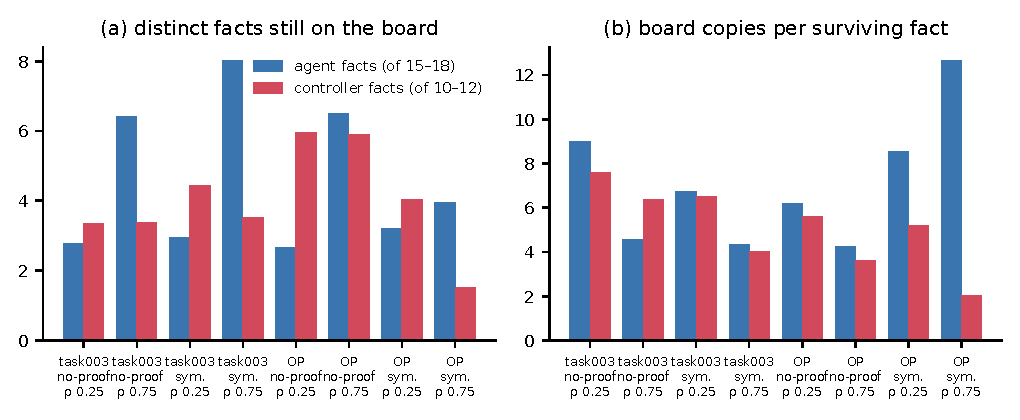
\includegraphics[width=\linewidth]{fig2_finite_sizes.pdf}
\caption{\textbf{Finite sizes in the simulator} at $t=30$ (false arm, $q=6$). (a) Distinct facts still on the board: most
of the agents' 15--18 facts have disappeared at short memory. (b) Board copies of each surviving fact: survivors are
concentrated in many copies.}
\label{fig:fs}
\end{figure}

\begin{result}[diversity collapse]
In a finite swarm, the agents' evidence does not thin out evenly. Most facts die out, and the survivors are held in many
copies. Shorter memory gives a stronger collapse: $F_{\rm eff}\approx3$ at $\rho=0.25$ against about 8 at $\rho=0.75$.
The relevant finite size is therefore not $N=24$ or $F_A=18$ separately. It is the number of surviving distinct facts
$F_{\rm eff}$, which depends on memory, reading and the copies per fact.
\end{result}

\paragraph{Why this matters for the two phenomena.} Each of these is a hypothesis to test in the finite version (next
steps):
\begin{itemize}
\item \textbf{Reversal.} Diversity collapse removes agents' own evidence mostly at short memory, which is where reading
  amplifies. It should therefore strengthen the amplifying side, and with it the size of $G$. The mean-field model's $G$
  is 3--10 times too small; this is a candidate reason.
\item \textbf{Proofs.} A proof needs specific facts. If they are extinct at short memory, no amount of reading can
  complete it. This sharpens the contrast between short and long memory in the symmetric setups.
\item \textbf{Persistence.} After the controller stops, the lasting damage (the residual after the controller's facts
  are removed) is exactly this lost diversity: agents' facts that died out do not come back.
\end{itemize}

\paragraph{How the sizes scale.} The effective sizes \eqref{eq:n}--\eqref{eq:F} explain two earlier scaling results:
\begin{itemize}
\item \textbf{Copying the same swarm $R$ times} (24$R$ agents, the same 18 facts) multiplies the copies per fact by $R$.
  Fewer facts die out, and the model approaches the mean field. This is what the earlier diagnostic found: $G$ fell from
  0.32 to 0.14 as $R$ went from 1 to 8.
\item \textbf{$K$ independent projects} (24$K$ agents and $K$ times as many facts) keep the copies per fact unchanged,
  so the collapse, and the finite-size effects, persist at every $K$.
\end{itemize}
So the theory's natural size parameter is the number of copies per fact, roughly $N/F$ and $W/F$, not $N$ alone.

\section{Next steps}
\label{sec:next}
\begin{enumerate}
\item \textbf{Test the $\beta_A$ explanation of the symmetric against no-proof crossover} (stored data, no new
  simulation, minutes).
  \begin{itemize}
  \item \emph{What:} measure, in each of the four setups, how much one more agent fact in memory lowers the exact belief
    in the wrong answer, $P(A2\mid M)$. This is an effective $\beta_A$: the slope of $\log$-odds of $A2$ against the
    number of agent facts held, from stored silent-arm memories.
  \item \emph{Prediction, fixed before measuring:} the effective $\beta_A$ is larger in the symmetric setups than in
    the no-proof ones, and the order of the four $\beta_A$ values matches the reverse order of the four crossovers
    (task003 no-proof 0.75--1, Object Placements no-proof 0.625--0.875, task003 symmetric 0.5--0.625, Object Placements
    symmetric 0.25--0.375).
  \item \emph{Then:} put the measured $\beta_A$ values into the model, without fitting anything else, and check whether
    the crossovers come out in the same order. If the order matches, the setup and task differences in the reversal
    are explained by one interpretable number. If not, that candidate is rejected.
  \end{itemize}
\item \textbf{A finite fact-flow model.}
  \begin{itemize}
  \item \emph{What:} the same equations, but with each fact's holders and board copies as whole numbers that can reach
    zero (a stochastic version, small: 16 agent facts, 4 controller facts, 24 agents, 48 posts).
  \item \emph{Predictions to test:}
    \begin{itemize}
    \item diversity collapse at short memory, as in Fig.~\ref{fig:fs};
    \item a larger controller effect $G$ than the mean field;
    \item a lasting residual after the controller's facts are removed;
    \item persistence that fades slowly over tens of time units, instead of reaching a plateau within 5--9.
    \end{itemize}
  \item \emph{Scaling check:} multiplying agents with fixed facts should approach the mean field; multiplying both
    should not.
  \end{itemize}
\item \textbf{A formula for the crossover} $\rho^*(q)$, from balancing the two terms of Eq.~\eqref{eq:D} in the
  short- and long-memory limits. It would explain why the crossover moves to shorter memory as reading grows.
\end{enumerate}

\end{document}
